\documentclass{article}
\usepackage[utf8]{inputenc}
\usepackage{enumitem}
\usepackage{graphicx}
\usepackage{tikz}

\begin{document}


\begin{titlepage}
    \centering
    \vspace*{2cm}
    {\Huge\bfseries Projet CMI: \par CYBER DEFENSE}
    \vspace{2cm}
    
    \begin{tikzpicture}[remember picture,overlay]
        \node[anchor=north west] at (current page.north west) {\LARGE
            \parbox[t]{1.0\textwidth}{
                Yassine LAMKADDEM \\
                Rémi AVOCAT\\
                Anaïs GUICCIARDI \\
                Lou RODRIGUEZ}};
        \node[anchor=north east] at (current page.north east) {\LARGE Groupe 9 / I};
        \node[anchor=south west] at (current page.south west) {\LARGE L1 INFO - CMI};
        \node[anchor=south east] at (current page.south east) {\LARGE 2023 - 2024};
    \end{tikzpicture}
    \begin{figure}[h]
        \centering
        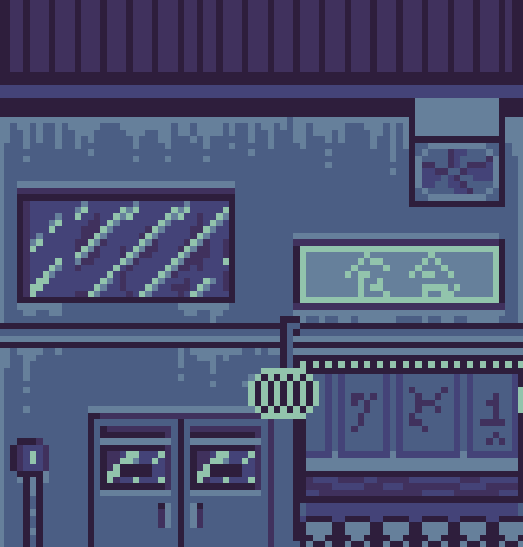
\includegraphics[width=0.8\textwidth]{page.png}
        \label{fig:page.png}
    \end{figure}
    
\end{titlepage}


\begin{center}
    \begin{minipage}{0.8\textwidth}
        \centering
        \hspace{0.8cm}
        {\LARGE\bfseries SOMMAIRE} \\[10pt]
        \begin{itemize}[label=-, itemsep=5pt]
            \item \large Introduction \hfill 2
            \item \large Mise en place du projet \hfill 2
            \begin{itemize}[label=--, font=\normalsize, itemsep=3pt]
                \item Objectifs du projet
                \item Organisation des idées
            \end{itemize}
            \item \large Réalisation du projet \hfill 3-4
            \begin{itemize}[label=--, font=\normalsize, itemsep=3pt]
                \item Choix du logiciel
                \item Éléments principaux du projet
            \item \large Gameplay \hfill 5
            \end{itemize}
            \item \large Conclusion \hfill 5
            % \item \large Manuel d’Utilisation \hfill 5
            \item \large Bibliographie \hfill 6
        \end{itemize}
    \end{minipage} 
\end{center}

\newpage

\setlength{\parindent}{1cm}

\section*{INTRODUCTION}
Un Tower defense est un genre de jeu vidéo où le joueur doit défendre une zone ou une base contre des vagues successives d'ennemis en plaçant des tours de défense chargées d’éliminer les assaillants. Le joueur doit ainsi tenir le plus longtemps possible en vie. Notre groupe (composé de Lou, Yassine, Rémi, Anais) a décidé à l’occasion du Projet L1 CMI 2024 de réaliser un jeu fonctionnel de ce genre. Ce projet nous permet de travailler notre cohésion de groupe, ce qui nous permet de développer nos compétences et notre expérience dans le domaine du développement informatique.

% Séparateur
\noindent 
\rule{\linewidth}{0.3mm}
%

\section*{MISE EN PLACE DU PROJET}
L’objectif principale est de réaliser un jeu “Top down view” dans lequel : 
\begin{itemize}
    \item Des ennemies arrivent par vague sur un même chemin 
    \item Le joueur peut placer des tours qui éliminent les ennemies 
    \item Présence d’une interface graphique utilisateur pour faciliter les actions du joueur.
\end{itemize}
\vspace{10pt}
Après une réflexion collective et en tenant compte de nos exigences , nous avons décidé de regrouper nos idées pour en faire une liste des différents éléments nécessaires à notre projet. 
Nous avons utilisé un graphique, offrant ainsi un outil visuel performant :

\begin{figure}[h]
    \centering
    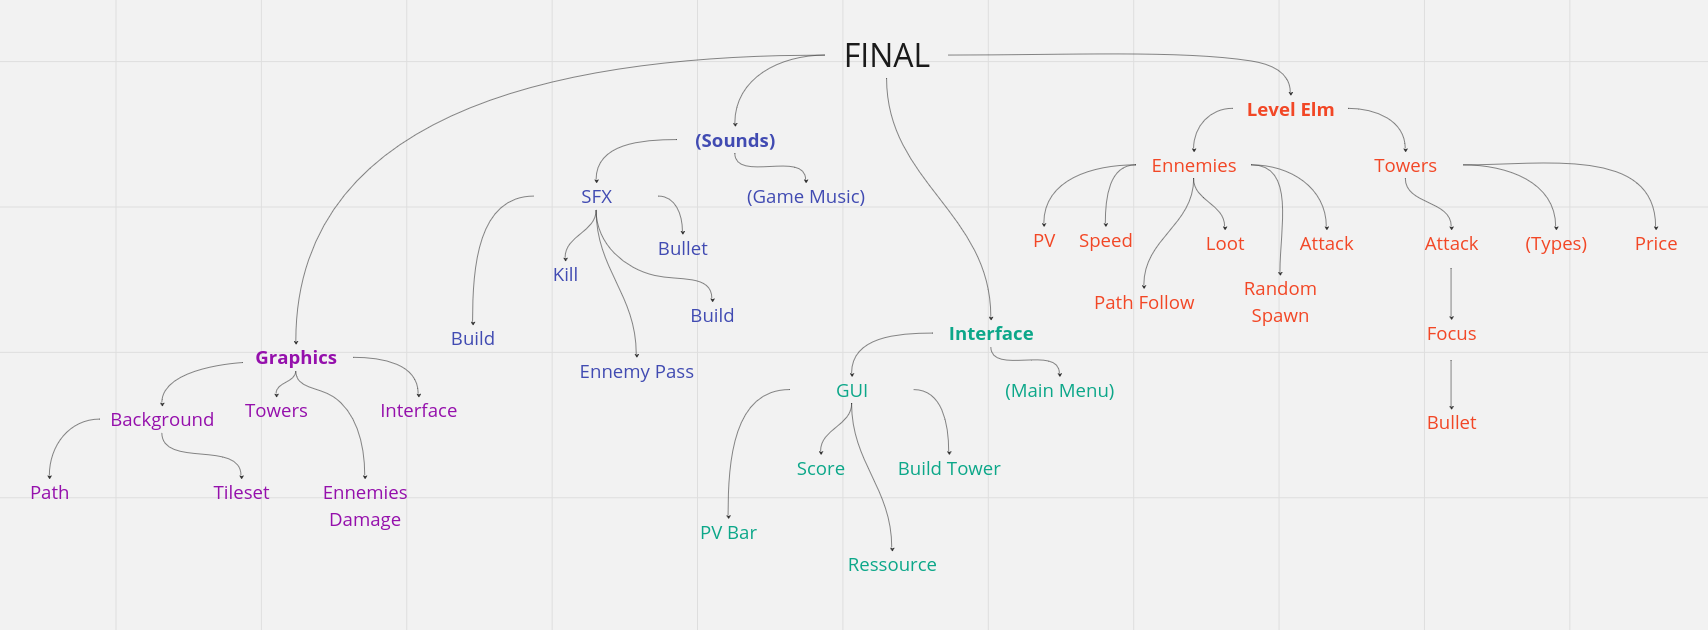
\includegraphics[width=1\textwidth]{arbre_elements_jeu.png}
    \caption{Arbre des différents éléments necessaires au fonctionnement du jeu, créé à l'aide de l'outil Miro.}
    \label{fig:arbre_elements_jeu.png}
\end{figure}

\newpage

\section*{RÉALISATION DU PROJET}

Afin de réaliser notre projet, nous avons décidé d’utiliser le logiciel “Godot”. Tout comme Unity ou encore Unreal Engine, “Godot Game Engine” est un moteur de jeu, c'est-à-dire un logiciel permettant de créer des jeux vidéo .
De plus, Il est multiplateforme, c'est-à dire qu’il est compatible à différents systèmes d'exploitation. Nous l’utiliserons sur linux et windows.
Godot possède son propre langage, le “GDscript” , sa syntaxe est similaire à celle de python, il possède une multitude de bibliothèque physique, 3D et 2D
dont certains s'avèreront essentiels à la réalisation de notre projet.
Nous visons en priorité un jeu fonctionnel sur PC mais il est possible grâce à Godot de l'exporter sur mobile. \par
\vspace{10pt}
\noindent Pour nous organiser, nous devions réaliser un diagramme de Gantt. Pour cela nous avons d’abord en présentiel rassembler nos tâches par catégorie. Ensuite nous en avons fait un tableau les classant par ordre de priorité, leur attribuant des dépendances à d’autres tâches et leur fixant une période max de travail.

\begin{figure}[h]
    \centering
    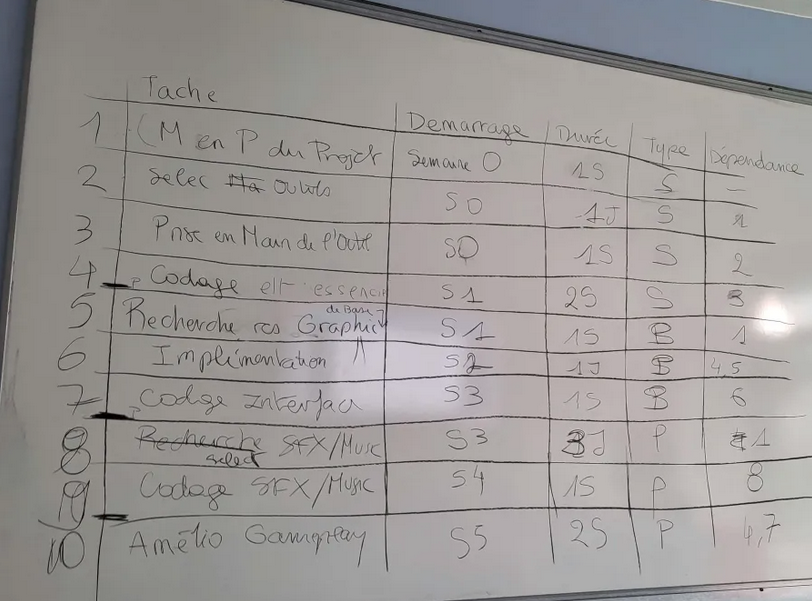
\includegraphics[width=1\textwidth]{tableau_pour_gantt.png}
    \label{fig:tableau_pour_gantt.png}
\end{figure}

\newpage

Il ne reste plus qu'à tracer notre diagramme à partir de ce tableau:
\vspace{-10pt}
\begin{figure}[h]
    \centering
    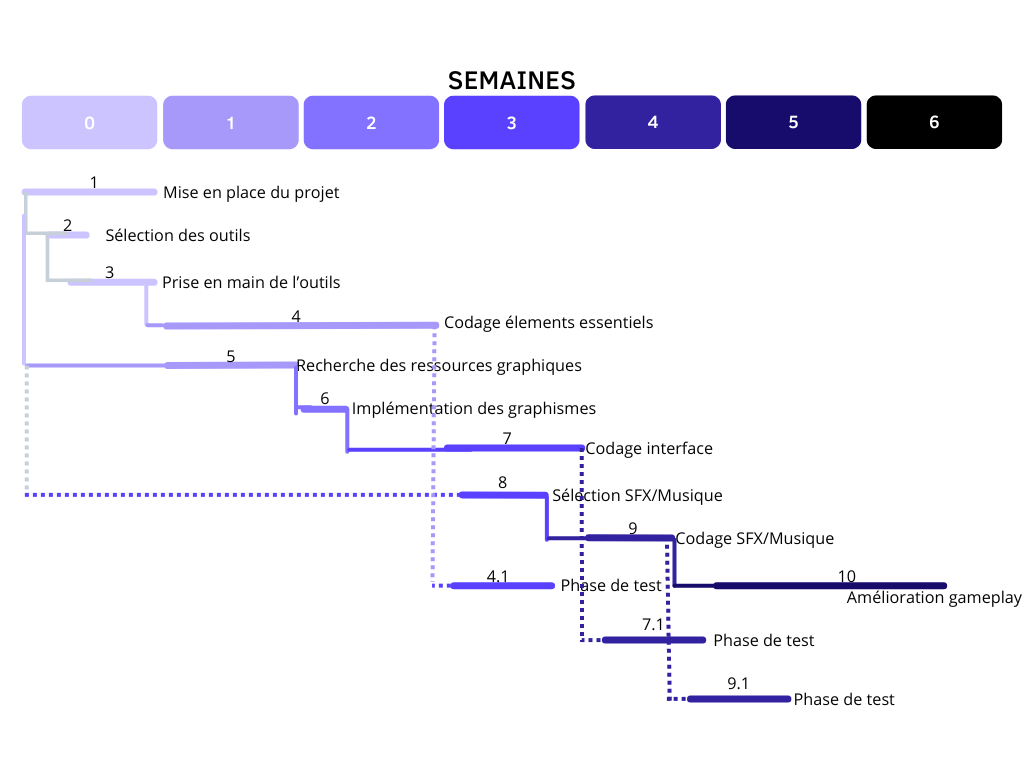
\includegraphics[width=1\textwidth]{diagram_gantt.png}
    \caption{Diagramme de Gantt de notre projet, créé à l'aide de l'outil Canva.}
    \label{fig:diagram_gantt.png}
\end{figure}

\noindent Maintenant que nous avons organisé notre travail dans le temps imparti et que nous avons choisi notre outil, nous pouvons commencer !

\newpage

\section*{GAMEPLAY}

\subsection*{Scénario}
Dans un futur cyberpunk, la police vient de débusquer la planque d'un jeune hacker. Le joueur se retrouve alors chargé de protéger ce repaire contre les assauts des forces de l'ordre.

\subsection*{Mécaniques de jeu}
Pour les mécaniques de jeu, nous resterons dans celles des tower defenses classiques : devoir se protéger d'ennemis suivant un chemin prédéfini à l’aide de défenses. Il faudra accumuler des ressources lâchées par les ennemis afin de construire de nouvelles défenses (tourelles), ou d'améliorer les actuelles (dans l'idéal, mais cette fonctionnalité n’est pas prioritaire). L’objectif est d'empêcher la police d’arriver au bout du chemin, dans le but de ne pas se faire arrêter. Pour que le jeu ne soit ni trop simple, ni trop dur, la difficulté augmente avec le temps, à l’aide d’un système de vagues, qui au fur et à mesure seront de plus en plus complexes (pour l’instant nous prévoyons juste d’augmenter le nombre d'ennemis, mais si nous avons le temps ce sera aussi en utilisant d’autres ennemis peut-être plus rapides, ou plus résistants …).

\subsection*{Interface Graphique}
Concernant l'interface graphique (GUI), nous prévoyons d'intégrer une barre de vie qui diminuera progressivement à mesure que la police atteigne la planque. Lorsque cette barre atteint 0, c'est le Game Over pour le joueur. De plus, nous inclurons un compteur d'argent pour permettre au joueur de gérer ses ressources et des emplacements de tour préétablis où il pourra placer ses défenses. Si le temps le permet, nous envisageons également d'ajouter un menu de démarrage pour faciliter la navigation et une page dédiée au Game Over pour une meilleure expérience utilisateur.
\subsection*{}
En fonction de l'évolution du projet, des ajustements ou des ajouts pourront être apportés.

\section*{Conclusion}
Nous avons planifié et allons réalisé un tower defense nommé “Cyber Défense” en 7 semaine sur le logiciel Godot en GDScript en équipe de 4(composé de Lou, Yassine, Rémi, Anais) pour le projet de second semestre L1 CMI .

% Séparateur
\noindent 

% \section*{MANUEL D'UTILISATION}

% \begin{itemize}
%     \item Itch.io → Recherche de ressources pour l’interface et le design général.
%     \item GitHub → Pour organiser notre code et pour que tout le groupe puisse y avoir accès et propose des changements.
%     \item OpenGameArt → Recherche de ressources pour le Sound Design (les musiques et les sons des effets spéciaux).
%     \item Documentation de Godot → Pour aider à coder et découvrir de nouvelles fonctionnalités du GDScript.
%     \item Miro et Canva → Pour faire facilement des schémas simples et compréhensibles.
%     \item LaTeX → Pour réaliser le cahier des charges ici présent.
% \end{itemize}

% % Séparateur
% \noindent 
% \rule{\linewidth}{0.3mm}
% %
\newpage


\section*{BIBLIOGRAPHIE}

\begin{itemize}
    \item Itch.io → Recherche de ressources pour l’interface et le design général.
    \item GitHub → Pour organiser notre code et pour que tout le groupe puisse y avoir accès et propose des changements.
    \item OpenGameArt → Recherche de ressources pour le Sound Design (les musiques et les sons des effets spéciaux).
    \item Documentation de Godot → Pour aider à coder et découvrir de nouvelles fonctionnalités du GDScript.
    \item Miro et Canva → Pour faire facilement des schémas simples et \par compréhensibles.
    \item LaTeX → Pour réaliser le cahier des charges ici présent.
\end{itemize}

\end{document}


